2050 Energistrategi
Den danske regering har skrevet under på, at Danmark til 2050 skal fuldstændig uafhængig af fossile brændsler. Det vil sige at Danmark skal være fri for kul, olie og naturgas, det betyder at Danmark vil satse på bæredygtig energiteknik, herunder vindenergi, bølgekraft og solceller. Herved er der også taget en del vindinitiativer, vi skal have 42\% af vores forbrug dækket af vindenergi inden 2020 (Se figur x).
\begin{figure}[H]
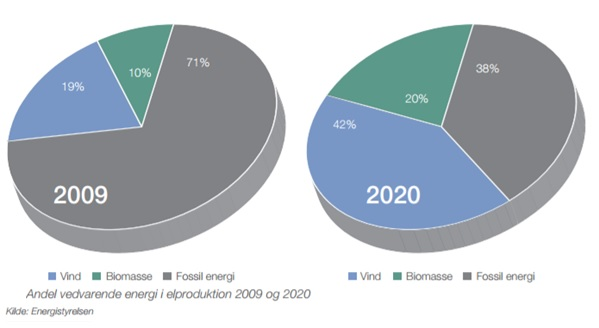
\includegraphics[scale=0.5]{Billeder/Cirkeldiagram_probana}
\end{figure}
For at man kan nå disse mål bliver Danmark nød til at bygge både vindmølleparker på land og på havet.
\begin{figure}[H]
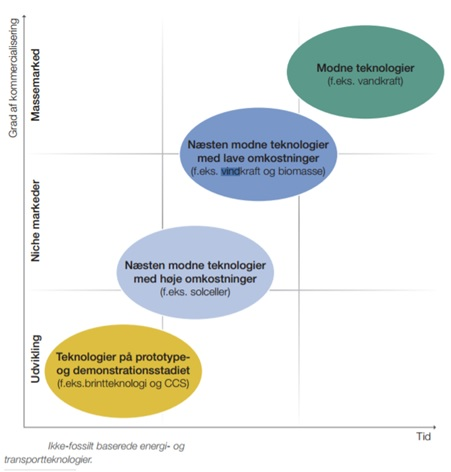
\includegraphics[scale=0.5]{Billeder/Baeredygtige_energiiniti}
\end{figure}
Vi kan se på figur X ovenfor at vand-, vindkraft og biomasse allerede er i/omkring massemarked så det er allerede muligheder som bliver brugt og videreudviklet. Imens solceller bliver solgt og stadig udviklet på. Brintteknologi er stadig kun i udviklingsfasen. 